\documentclass[11pt]{article}
\usepackage[OT4]{fontenc}
\newtheorem{define}{Definition}
\usepackage{graphicx}
\usepackage{subcaption}
\usepackage{hyperref}
\usepackage{booktabs}
\oddsidemargin=0.15in
\evensidemargin=0.15in
\topmargin=-.5in
\textheight=9in
\textwidth=6.25in

\begin{document}
	
%--------------
%% preamble.tex
%% this should be included with a command like
%% %--------------
%% preamble.tex
%% this should be included with a command like
%% %--------------
%% preamble.tex
%% this should be included with a command like
%% \input{preamble.tex}
%% Template based on Aleksander Madry's and Dan Spielman's template

\hbadness=10000
\vbadness=10000

\setlength{\oddsidemargin}{.25in}
\setlength{\evensidemargin}{.25in}
\setlength{\textwidth}{6in}
\setlength{\topmargin}{-0.4in}
\setlength{\textheight}{8.5in}

\newcommand{\handout}[5]{
	\noindent
	\begin{center}
		\framebox{
			\vbox{
				\hbox to 5.78in { {\bf #1}
					\hfill #2 }
				\vspace{4mm}
				\hbox to 5.78in { {\Large \hfill #5  \hfill} }
				\vspace{2mm}
				\hbox to 5.78in { {\it #3 \hfill #4} }
			}
		}
	\end{center}
	\vspace*{4mm}
}

\newcommand{\header}[2]{\handout{NUS CS4243: Computer Vision and Pattern Recognition}{\today}{Lecturer: Angela Yao;}{Students: #1}{#2}}


\newtheorem{theorem}{Theorem}
\newtheorem{corollary}[theorem]{Corollary}
\newtheorem{lemma}[theorem]{Lemma}
\newtheorem{observation}[theorem]{Observation}
\newtheorem{proposition}[theorem]{Proposition}
\newtheorem{definition}[theorem]{Definition}
\newtheorem{claim}[theorem]{Claim}
\newtheorem{fact}[theorem]{Fact}
\newtheorem{assumption}[theorem]{Assumption}

\newcommand{\qed}{\rule{7pt}{7pt}}
\newcommand{\dis}{\mathop{\mbox{\rm d}}\nolimits}
\newcommand{\per}{\mathop{\mbox{\rm per}}\nolimits}
\newcommand{\area}{\mathop{\mbox{\rm area}}\nolimits}
\newcommand{\cw}{\mathop{\rm cw}\nolimits}
\newcommand{\ccw}{\mathop{\rm ccw}\nolimits}
\newcommand{\DIST}{\mathop{\mbox{\rm DIST}}\nolimits}
\newcommand{\OP}{\mathop{\mbox{\it OP}}\nolimits}
\newcommand{\OPprime}{\mathop{\mbox{\it OP}^{\,\prime}}\nolimits}
\newcommand{\ihat}{\hat{\imath}}
\newcommand{\jhat}{\hat{\jmath}}
\newcommand{\abs}[1]{\mathify{\left| #1 \right|}}

\newenvironment{proof}{\noindent{\bf Proof}\hspace*{1em}}{\qed\bigskip}
\newenvironment{proof-sketch}{\noindent{\bf Sketch of Proof}\hspace*{1em}}{\qed\bigskip}
\newenvironment{proof-idea}{\noindent{\bf Proof Idea}\hspace*{1em}}{\qed\bigskip}
\newenvironment{proof-of-lemma}[1]{\noindent{\bf Proof of Lemma #1}\hspace*{1em}}{\qed\bigskip}
\newenvironment{proof-attempt}{\noindent{\bf Proof Attempt}\hspace*{1em}}{\qed\bigskip}
\newenvironment{proofof}[1]{\noindent{\bf Proof}
of #1:\hspace*{1em}}{\qed\bigskip}
\newenvironment{remark}{\noindent{\bf Remark}\hspace*{1em}}{\bigskip}

% \makeatletter
% \@addtoreset{figure}{section}
% \@addtoreset{table}{section}
% \@addtoreset{equation}{section}
% \makeatother

\newcommand{\FOR}{{\bf for}}
\newcommand{\TO}{{\bf to}}
\newcommand{\DO}{{\bf do}}
\newcommand{\WHILE}{{\bf while}}
\newcommand{\AND}{{\bf and}}
\newcommand{\IF}{{\bf if}}
\newcommand{\THEN}{{\bf then}}
\newcommand{\ELSE}{{\bf else}}

% \renewcommand{\thefigure}{\thesection.\arabic{figure}}
% \renewcommand{\thetable}{\thesection.\arabic{table}}
% \renewcommand{\theequation}{\thesection.\arabic{equation}}

\makeatletter
\def\fnum@figure{{\bf Figure \thefigure}}
\def\fnum@table{{\bf Table \thetable}}
\long\def\@mycaption#1[#2]#3{\addcontentsline{\csname
  ext@#1\endcsname}{#1}{\protect\numberline{\csname 
  the#1\endcsname}{\ignorespaces #2}}\par
  \begingroup
    \@parboxrestore
    \small
    \@makecaption{\csname fnum@#1\endcsname}{\ignorespaces #3}\par
  \endgroup}
\def\mycaption{\refstepcounter\@captype \@dblarg{\@mycaption\@captype}}
\makeatother

\newcommand{\figcaption}[1]{\mycaption[]{#1}}
\newcommand{\tabcaption}[1]{\mycaption[]{#1}}
\newcommand{\head}[1]{\chapter[Lecture \##1]{}}
\newcommand{\mathify}[1]{\ifmmode{#1}\else\mbox{$#1$}\fi}
%\renewcommand{\Pr}[1]{\mathify{\mbox{Pr}\left[#1\right]}}
%\newcommand{\Exp}[1]{\mathify{\mbox{Exp}\left[#1\right]}}
\newcommand{\bigO}O
\newcommand{\set}[1]{\mathify{\left\{ #1 \right\}}}
\def\half{\frac{1}{2}}

\newcommand{\fig}[4]{
        \begin{figure}
        \setlength{\epsfysize}{#2}
        \vspace{3mm}
        \centerline{\epsfbox{#4}}
        \caption{#3} \label{#1}
        \end{figure}
        }

\newcommand{\ord}{{\rm ord}}

\providecommand{\norm}[1]{\lVert #1 \rVert}
\newcommand{\embed}{{\rm Embed}}
\newcommand{\qembed}{\mbox{$q$-Embed}}
\newcommand{\calh}{{\cal H}}
\newcommand{\lp}{{\rm LP}}

%% Template based on Aleksander Madry's and Dan Spielman's template

\hbadness=10000
\vbadness=10000

\setlength{\oddsidemargin}{.25in}
\setlength{\evensidemargin}{.25in}
\setlength{\textwidth}{6in}
\setlength{\topmargin}{-0.4in}
\setlength{\textheight}{8.5in}

\newcommand{\handout}[5]{
	\noindent
	\begin{center}
		\framebox{
			\vbox{
				\hbox to 5.78in { {\bf #1}
					\hfill #2 }
				\vspace{4mm}
				\hbox to 5.78in { {\Large \hfill #5  \hfill} }
				\vspace{2mm}
				\hbox to 5.78in { {\it #3 \hfill #4} }
			}
		}
	\end{center}
	\vspace*{4mm}
}

\newcommand{\header}[2]{\handout{NUS CS4243: Computer Vision and Pattern Recognition}{\today}{Lecturer: Angela Yao;}{Students: #1}{#2}}


\newtheorem{theorem}{Theorem}
\newtheorem{corollary}[theorem]{Corollary}
\newtheorem{lemma}[theorem]{Lemma}
\newtheorem{observation}[theorem]{Observation}
\newtheorem{proposition}[theorem]{Proposition}
\newtheorem{definition}[theorem]{Definition}
\newtheorem{claim}[theorem]{Claim}
\newtheorem{fact}[theorem]{Fact}
\newtheorem{assumption}[theorem]{Assumption}

\newcommand{\qed}{\rule{7pt}{7pt}}
\newcommand{\dis}{\mathop{\mbox{\rm d}}\nolimits}
\newcommand{\per}{\mathop{\mbox{\rm per}}\nolimits}
\newcommand{\area}{\mathop{\mbox{\rm area}}\nolimits}
\newcommand{\cw}{\mathop{\rm cw}\nolimits}
\newcommand{\ccw}{\mathop{\rm ccw}\nolimits}
\newcommand{\DIST}{\mathop{\mbox{\rm DIST}}\nolimits}
\newcommand{\OP}{\mathop{\mbox{\it OP}}\nolimits}
\newcommand{\OPprime}{\mathop{\mbox{\it OP}^{\,\prime}}\nolimits}
\newcommand{\ihat}{\hat{\imath}}
\newcommand{\jhat}{\hat{\jmath}}
\newcommand{\abs}[1]{\mathify{\left| #1 \right|}}

\newenvironment{proof}{\noindent{\bf Proof}\hspace*{1em}}{\qed\bigskip}
\newenvironment{proof-sketch}{\noindent{\bf Sketch of Proof}\hspace*{1em}}{\qed\bigskip}
\newenvironment{proof-idea}{\noindent{\bf Proof Idea}\hspace*{1em}}{\qed\bigskip}
\newenvironment{proof-of-lemma}[1]{\noindent{\bf Proof of Lemma #1}\hspace*{1em}}{\qed\bigskip}
\newenvironment{proof-attempt}{\noindent{\bf Proof Attempt}\hspace*{1em}}{\qed\bigskip}
\newenvironment{proofof}[1]{\noindent{\bf Proof}
of #1:\hspace*{1em}}{\qed\bigskip}
\newenvironment{remark}{\noindent{\bf Remark}\hspace*{1em}}{\bigskip}

% \makeatletter
% \@addtoreset{figure}{section}
% \@addtoreset{table}{section}
% \@addtoreset{equation}{section}
% \makeatother

\newcommand{\FOR}{{\bf for}}
\newcommand{\TO}{{\bf to}}
\newcommand{\DO}{{\bf do}}
\newcommand{\WHILE}{{\bf while}}
\newcommand{\AND}{{\bf and}}
\newcommand{\IF}{{\bf if}}
\newcommand{\THEN}{{\bf then}}
\newcommand{\ELSE}{{\bf else}}

% \renewcommand{\thefigure}{\thesection.\arabic{figure}}
% \renewcommand{\thetable}{\thesection.\arabic{table}}
% \renewcommand{\theequation}{\thesection.\arabic{equation}}

\makeatletter
\def\fnum@figure{{\bf Figure \thefigure}}
\def\fnum@table{{\bf Table \thetable}}
\long\def\@mycaption#1[#2]#3{\addcontentsline{\csname
  ext@#1\endcsname}{#1}{\protect\numberline{\csname 
  the#1\endcsname}{\ignorespaces #2}}\par
  \begingroup
    \@parboxrestore
    \small
    \@makecaption{\csname fnum@#1\endcsname}{\ignorespaces #3}\par
  \endgroup}
\def\mycaption{\refstepcounter\@captype \@dblarg{\@mycaption\@captype}}
\makeatother

\newcommand{\figcaption}[1]{\mycaption[]{#1}}
\newcommand{\tabcaption}[1]{\mycaption[]{#1}}
\newcommand{\head}[1]{\chapter[Lecture \##1]{}}
\newcommand{\mathify}[1]{\ifmmode{#1}\else\mbox{$#1$}\fi}
%\renewcommand{\Pr}[1]{\mathify{\mbox{Pr}\left[#1\right]}}
%\newcommand{\Exp}[1]{\mathify{\mbox{Exp}\left[#1\right]}}
\newcommand{\bigO}O
\newcommand{\set}[1]{\mathify{\left\{ #1 \right\}}}
\def\half{\frac{1}{2}}

\newcommand{\fig}[4]{
        \begin{figure}
        \setlength{\epsfysize}{#2}
        \vspace{3mm}
        \centerline{\epsfbox{#4}}
        \caption{#3} \label{#1}
        \end{figure}
        }

\newcommand{\ord}{{\rm ord}}

\providecommand{\norm}[1]{\lVert #1 \rVert}
\newcommand{\embed}{{\rm Embed}}
\newcommand{\qembed}{\mbox{$q$-Embed}}
\newcommand{\calh}{{\cal H}}
\newcommand{\lp}{{\rm LP}}

%% Template based on Aleksander Madry's and Dan Spielman's template

\hbadness=10000
\vbadness=10000

\setlength{\oddsidemargin}{.25in}
\setlength{\evensidemargin}{.25in}
\setlength{\textwidth}{6in}
\setlength{\topmargin}{-0.4in}
\setlength{\textheight}{8.5in}

\newcommand{\handout}[5]{
	\noindent
	\begin{center}
		\framebox{
			\vbox{
				\hbox to 5.78in { {\bf #1}
					\hfill #2 }
				\vspace{4mm}
				\hbox to 5.78in { {\Large \hfill #5  \hfill} }
				\vspace{2mm}
				\hbox to 5.78in { {\it #3 \hfill #4} }
			}
		}
	\end{center}
	\vspace*{4mm}
}

\newcommand{\header}[2]{\handout{NUS CS4243: Computer Vision and Pattern Recognition}{\today}{Lecturer: Angela Yao;}{Students: #1}{#2}}


\newtheorem{theorem}{Theorem}
\newtheorem{corollary}[theorem]{Corollary}
\newtheorem{lemma}[theorem]{Lemma}
\newtheorem{observation}[theorem]{Observation}
\newtheorem{proposition}[theorem]{Proposition}
\newtheorem{definition}[theorem]{Definition}
\newtheorem{claim}[theorem]{Claim}
\newtheorem{fact}[theorem]{Fact}
\newtheorem{assumption}[theorem]{Assumption}

\newcommand{\qed}{\rule{7pt}{7pt}}
\newcommand{\dis}{\mathop{\mbox{\rm d}}\nolimits}
\newcommand{\per}{\mathop{\mbox{\rm per}}\nolimits}
\newcommand{\area}{\mathop{\mbox{\rm area}}\nolimits}
\newcommand{\cw}{\mathop{\rm cw}\nolimits}
\newcommand{\ccw}{\mathop{\rm ccw}\nolimits}
\newcommand{\DIST}{\mathop{\mbox{\rm DIST}}\nolimits}
\newcommand{\OP}{\mathop{\mbox{\it OP}}\nolimits}
\newcommand{\OPprime}{\mathop{\mbox{\it OP}^{\,\prime}}\nolimits}
\newcommand{\ihat}{\hat{\imath}}
\newcommand{\jhat}{\hat{\jmath}}
\newcommand{\abs}[1]{\mathify{\left| #1 \right|}}

\newenvironment{proof}{\noindent{\bf Proof}\hspace*{1em}}{\qed\bigskip}
\newenvironment{proof-sketch}{\noindent{\bf Sketch of Proof}\hspace*{1em}}{\qed\bigskip}
\newenvironment{proof-idea}{\noindent{\bf Proof Idea}\hspace*{1em}}{\qed\bigskip}
\newenvironment{proof-of-lemma}[1]{\noindent{\bf Proof of Lemma #1}\hspace*{1em}}{\qed\bigskip}
\newenvironment{proof-attempt}{\noindent{\bf Proof Attempt}\hspace*{1em}}{\qed\bigskip}
\newenvironment{proofof}[1]{\noindent{\bf Proof}
of #1:\hspace*{1em}}{\qed\bigskip}
\newenvironment{remark}{\noindent{\bf Remark}\hspace*{1em}}{\bigskip}

% \makeatletter
% \@addtoreset{figure}{section}
% \@addtoreset{table}{section}
% \@addtoreset{equation}{section}
% \makeatother

\newcommand{\FOR}{{\bf for}}
\newcommand{\TO}{{\bf to}}
\newcommand{\DO}{{\bf do}}
\newcommand{\WHILE}{{\bf while}}
\newcommand{\AND}{{\bf and}}
\newcommand{\IF}{{\bf if}}
\newcommand{\THEN}{{\bf then}}
\newcommand{\ELSE}{{\bf else}}

% \renewcommand{\thefigure}{\thesection.\arabic{figure}}
% \renewcommand{\thetable}{\thesection.\arabic{table}}
% \renewcommand{\theequation}{\thesection.\arabic{equation}}

\makeatletter
\def\fnum@figure{{\bf Figure \thefigure}}
\def\fnum@table{{\bf Table \thetable}}
\long\def\@mycaption#1[#2]#3{\addcontentsline{\csname
  ext@#1\endcsname}{#1}{\protect\numberline{\csname 
  the#1\endcsname}{\ignorespaces #2}}\par
  \begingroup
    \@parboxrestore
    \small
    \@makecaption{\csname fnum@#1\endcsname}{\ignorespaces #3}\par
  \endgroup}
\def\mycaption{\refstepcounter\@captype \@dblarg{\@mycaption\@captype}}
\makeatother

\newcommand{\figcaption}[1]{\mycaption[]{#1}}
\newcommand{\tabcaption}[1]{\mycaption[]{#1}}
\newcommand{\head}[1]{\chapter[Lecture \##1]{}}
\newcommand{\mathify}[1]{\ifmmode{#1}\else\mbox{$#1$}\fi}
%\renewcommand{\Pr}[1]{\mathify{\mbox{Pr}\left[#1\right]}}
%\newcommand{\Exp}[1]{\mathify{\mbox{Exp}\left[#1\right]}}
\newcommand{\bigO}O
\newcommand{\set}[1]{\mathify{\left\{ #1 \right\}}}
\def\half{\frac{1}{2}}

\newcommand{\fig}[4]{
        \begin{figure}
        \setlength{\epsfysize}{#2}
        \vspace{3mm}
        \centerline{\epsfbox{#4}}
        \caption{#3} \label{#1}
        \end{figure}
        }

\newcommand{\ord}{{\rm ord}}

\providecommand{\norm}[1]{\lVert #1 \rVert}
\newcommand{\embed}{{\rm Embed}}
\newcommand{\qembed}{\mbox{$q$-Embed}}
\newcommand{\calh}{{\cal H}}
\newcommand{\lp}{{\rm LP}}

\header{Maximilian Fruehauf, David Drews, Choo Wen Xin}{Where's Waldo Detector using Computer Vision}
\begin{abstract}
This report describes our group's implementation of a computer vision algorithm to detect Waldo, Wenda, and the Wizard from a series of "Where's Waldo" books. The goal of this project is to detect the three characters from the provided high-resolution images, which can be very complex with a lot of detail and many other characters. The three characters also may or may not appear in any given image.\\

Due to the complex nature of the given images, and variation of the characters' appearances, detecting the characters accurately proved to be a challenge. In some cases, we could not identify where the characters are, and a lot of false positives were present as well.\\

Our proposed solution is to use a histogrammed feature descriptor, then training a linear support vector machine (SVM) to create our classifier. We were able to detect some instances of Waldo, espcially in the postcard in the top left hand corner of the page.


\end{abstract}
%%%% body goes in here %%%%
\section{Introduction}


"Where's Waldo" is a series of books containing detailed, high-resolution illustrations. For this project, we are given a set of scanned images from the book, and are tasked to design a computer vision algorithm that can detect the three characters from the book: Waldo, Wenda, and the Wizard. Each image may contain one or more of these characters. We are provided with a set of training images with annotations of the bounding box locations of Waldo, Wenda, or the Wizard in each image.\\

Throughout the course of the project, we have attempted several different methods with varying degrees of success. 
While there are several existing computer vision algorithms for face and object detection, 
such as the YOLO (You Only Look Once) by Redmon et. al. \cite{redmon2016yolo}, these modern approaches
all use Deep Convolutional Neutral Networks, which we were not allowed to use. Therefore we were looking for a "Non-Deep" method.
The characters' appearance and size also seems to vary across images, sometimes only a smaller part of the character (i.e a part of the face) is visible. This makes identifying the characters more challenging as well.\\

Across all approaches, we've only been working with the data that was handed to us as part of the assignment. Although our code alters the given data wherever needed, we did neither add any entirely new data from sources like the internet nor did we manually improve the existing data as could be achieved by adding or improving annotations.\\

The data we utilised can be summarised as follows:

\begin{itemize}
    \item 80 high resolution images from the \textit{Where's Waldo} book series
    \item 137 images of Waldo cropped to the patch of the image as describe in the annotation files
    \item 43 images of Wenda cropped to the patch of the image as describe in the annotation files
    \item 27 images of Wizard cropped to the patch of the image as describe in the annotation files
    \item Approximately 14,000 to 15,000 images (128x128px) subsampled from the original images, which did neither contain Waldo, Wenda or Wizard, used as negative training samples
\end{itemize}

In order to assess the performance of our algorithms we split the given set of images in a training and a testing set. This reduced the amount of positive samples of the three characters to 124 training samples for Waldo, 36 for Wenda and 24 for Wizard. As we will discuss in the upcoming sections, this uneaven split of training samples influenced the performance of our solution for the three different classes. 

We proposed using a few methods:

\begin{itemize}
    \item histogram over gradients (HoG) feature descriptor
    \item histogram over values (HoV) feature descriptor
    \item training a linear support vector machine (SVM) to create a multiclass-classifier
\end{itemize}

We will discuss our proposed solution in the next section.\\

\begin{figure}[h]
    \centering
    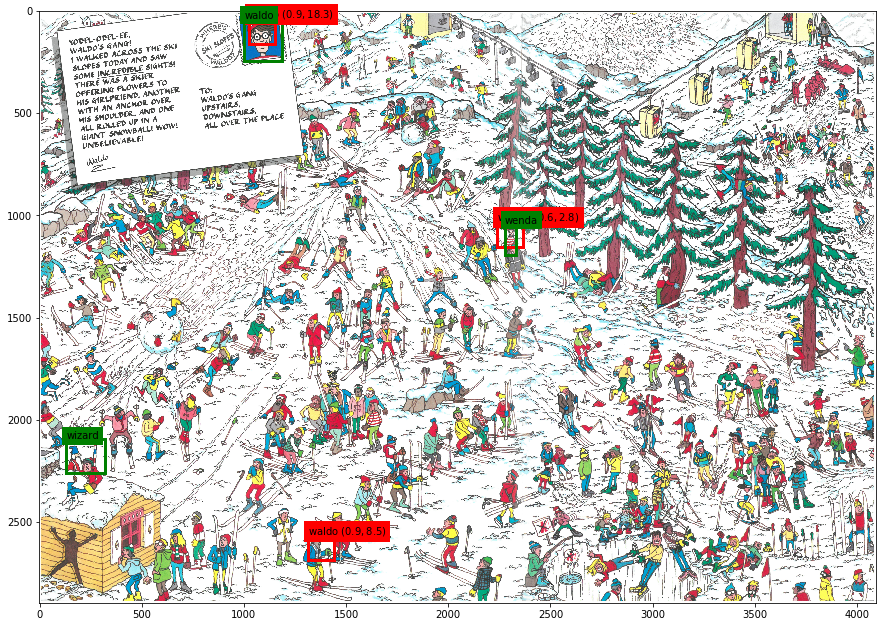
\includegraphics[width=0.9\linewidth]{figures/waldo_winter} 
    \caption{Exmaple of an image showing detections with \( (name, p, p_{ratio}) \) in red, ground truth in green}
    \label{fig:waldo-winter}
\end{figure}

\section{Proposed Solution}
Our proposed solution has two phases: pre-processing and detection.

\begin{figure}[h]
    \centering
    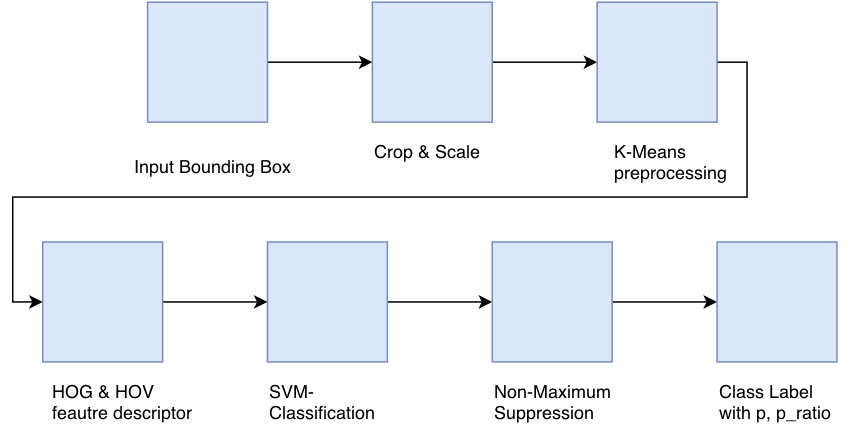
\includegraphics[width=0.9\linewidth]{figures/model_overview} 
    \caption{Schematic overview of the wlado / wenda / wizard detection pileline.}
    \label{fig:model-overview}
\end{figure}

In the pre-processing phase, we will take all the provided high-resolution training images and crop out the three characters using the given input bounding box annotations. Negative samples will be obtained by arbitiarily sampling regions from the images that do not overlap with the given character bounding boxes. We will scale all these images to a fixed size for simplification. We will then run k-means preprocessing on these images to map the colored sample images to grayscale values.

The details will be further discussed in \autoref{subsec:data-prep}\\

Our detection phase first involves histogramming two types of feature descriptors: gradients (HoG) and values (HoV).

HoG will be used to histogram horizontal and vertical gradients in the image, which could be quite helpful in identifying features like the horizontal stripes in Waldo and Wenda's shirts. HoV is to histogram values from a SIFT detector.

We will use our training samples to train support vector machines (SVM) as a classifier to determine whether a window is either \(Waldo, Wenda, Wizard or Negative\). The classifier will predict a probability \(p\) that a window belongs to a certain class, and a ratio \(p_ratio\) to indicate the classifier's confidence in ratio to the other classes.

Afterwhich, we will perform non-maximum supression to rermove overlapping windows by choosing the one with the highest probability in each group.

Finally, the resulting boxes with the class label will be drawn on the image with the value of its probability and ratio.

The details will be further discussed in \autoref{subsec:implementation}\\


\section{Experiments}
\subsection{Data Preparation and Configuration}\label{subsec:data-prep}

The images in the dataset come as annotated bounding boxes of varying aspect ratios and sizes in pixels.
Also the size of the respective images changes as well. Therefore we simplified the detection process by
generating \( (128 \times 128) \) px training images from the provided bounding boxes. 
Doing so resulted in some cropping to the actual characters appearances, which cannot be avoided in some corner cases.
However, in general we were able to regularize the bounding boxes without losing any pixels belonging to the positive annotations.
See \autoref{fig:preprocessed-samples} for examples of the cropped and scaled input images.

\begin{figure}[h]
    \centering
    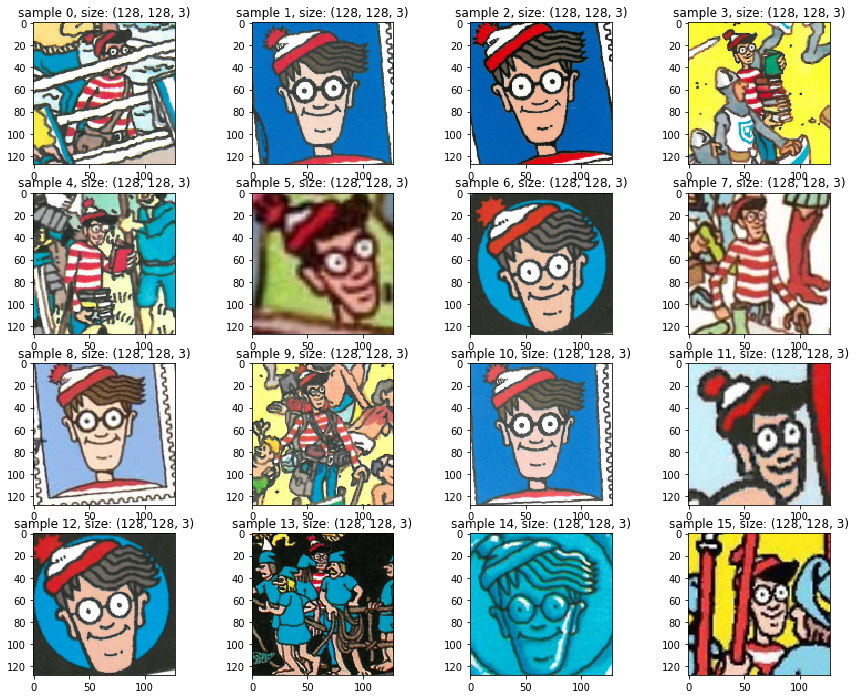
\includegraphics[width=0.4\linewidth]{figures/preprocess_waldo} 
    \hspace{1cm}
    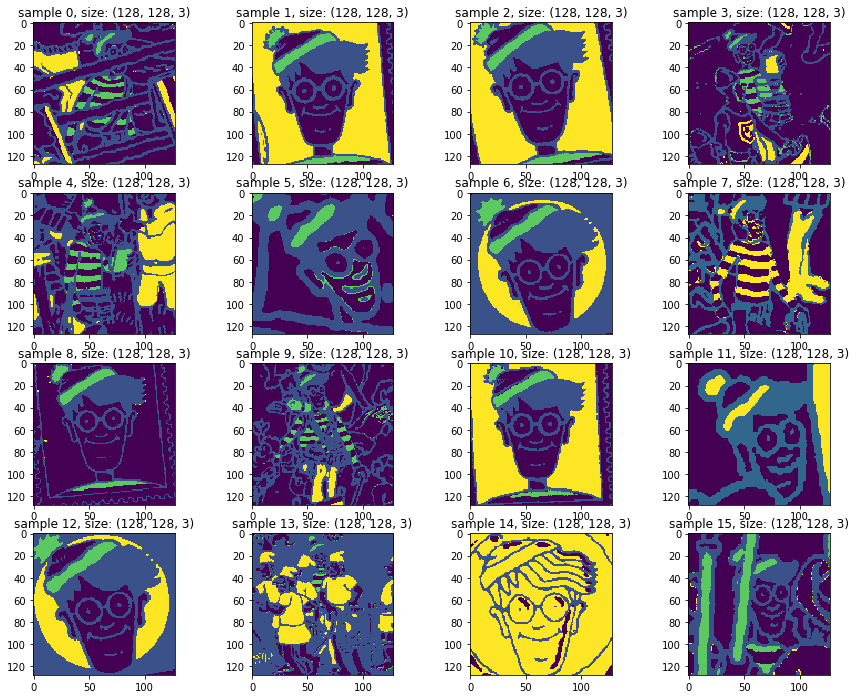
\includegraphics[width=0.4\linewidth]{figures/kmeans_waldo} 
    \caption{Preprocessed sample images for the waldo class. The left images are cropped and scaled to \( 128 \times 128 \) pixels.
    To the right the same images are shown after kemans preprocessing (originally gray-scale, but color mapped for display purposes)}
    \label{fig:preprocessed-samples}
\end{figure}

To map the color images as robustly as possible to gray scale values we used a K-Means detector 
and assigned each of the modes an equally gray spaced color. 
K-Means works by intially choosing random starting points in the image and then projecting an area around them, calculating the "center of gravity"
of those inlier points and then shifting the new centroid to this "center of gravity". When repeating this
process until convergence, \( k \) such different means are found. This process results in a non-uniform quantization of the input image.

We use this property to train the K-Means classifier on a sample image of the \verb|wenda| class, which only 
shows the colors red, blue, black white. However we use \( k=5 \) to classify any color not lying in these four as a separate class, and then merge 
its results with the white color class. Then these four resulting classes colored centroids are mapped to uniformly
chosen values \( v \in [0, 255] \). This drastically reduces the complexity of the input images as can be seen in the right image in \autoref{fig:preprocessed-samples},
reducing input noise when processing the images with our feature descriptor in \autoref{subsec:implementation}.

\vspace{0.5cm}
Generating negative samples is done by randomly sampling regions of differing scales and positions from the provided training images.
In this process we additionally make sure that none of the proposed negative samples overlap with any of the ground truth annotations present in the images.
Then we scale these proposed negative samples to \( (128 \times 128 ) \) px and apply the filtering described in the above paragraph to each sample.
Since the negative samples are randomly generated, we can create arbitrary amounts of them. 
For our testing \( \approx15000 \) worked well. 
Additonal information in the exact size of the dataset is shown in \autoref{tab:dataset-stats}

\begin{table}[]
    \centering
    \begin{tabular}{ccc}
        \toprule
        Class name & \#samples & percentage \\
        \midrule
        waldo & 137 &  1.01\% \\
        wenda & 43&  0.32\% \\
        wizard& 27&  0.20\% \\
        negative & 13315&  98.47\% \\
        \bottomrule
    \end{tabular}
    \caption{Dataset statistics for the training}
    \label{tab:dataset-stats}
\end{table}


\subsection{Implementation}\label{subsec:implementation}

The pipeline for detecting the classes of a given bounding box are displayed in \autoref{fig:model-overview},
the first 3 steps of which are covered in \autoref{subsec:data-prep}. In the following paragraps we will focus on the
steps 4-7 of any detection and provide some details of interest in the implementation.

\paragraph{HOG \& HOV feauture descriptor}
To capture shape and color information from the preprocessed sample images, we adopt a twofold feature descriptor, 
which consists of the HOG descriptor and a histogramed version of the SIFT detector, we call HOV.

HOG works by first calculating the horizontal and vertical gradients in the image, which are then separated into
quadratic cells. From both a horizontal and vertical window, the magnitude and direction (radians or degrees) of the gradient get computed.
Then the magnitude is binned according to the corresponding direction. These bins then form a histogram for the cell.
This gives some invariance of the feature descriptor to slight pixel value changes. 
To also gives some spatial invariance, a set number of these histogramed cells are concatenated together. Which is repeated for each cell.
In a final step, the resulting feature vector is normalized with one of a multitude of possible norms. We decided to use the \( L_2 \)-Hys norm.

The HOV (Histograms over Values) descriptor works essentially the same (in fact most of the code is copied from the \verb|scikit-image| HOG implemenation),
with the only difference being that the initial histogram on each cell is not computed from the gradient of the input,
but rather the values of the input image inself.

Concatenating these two independently (with the same parameters) computed feature descriptors gives a good spatial and
value representation of the input images. The effect of which we evaluate in \autoref{subsec:results}.


\paragraph{SVM Classification}
Deciding which of the four classes \( \{waldo, wenda, wizard, negative \} \) should be assigned to any given window 
as confidently as possible, is handled by an ensemble of SVMs (Support Vector Machine)\cite{Hearst:1998:SVM:630302.630387}.

One SVM can only be used as a binary classifier, as explained in the remainder of this paragraph, but we require multiclass classification. 
Therefore we adopt a one-vs-one classification approach, where for each pair of classes \( \forall i,j: (c_i,c_j) \) a separate binary classifier is trained
and classifications are chosen by majority vote. We chose a one-vs-one approach versus a more traditional one-vs-rest approach as we a very unequal distribution of
positive an negative samples. Therefore any one-vs-rest classifier learns to only differentiate between the given class and negative samples. This showed itself 
during testing and classification performance could be improved by switching to a one-vs-one approach, even considering the additional computational expense.

Any one of the trained SVMs works by finding a hyperplane (plane in high dimensional feature space) which best separates the positive, from the negative samples.
The computation of this plane is performed iteratively by choosing a random starting plane and then finding dimensions which provide a good separation of the data. 
One such "good" separation is called a support vector of the hyperplane, giving the name Support Vector Machine. 
However this only works well if the data can be linearly separated by the dimensions of the input data. 
Since this is not always the case, and in general hard to analyse in high dimensional cases, we adopt an approach called RBF (Radial basis function) as proposed in\cite{10.1007/978-3-540-28647-9_85}.
Wang et. al. use this radial basis function to extend the data into another dimension, which in which it is hopefully linearly separable. Fitting this RBF kernel is also done at training time.
Traditionally SVMs can only give a distance of the sample from the decision hyperplane as a measure of confidence. 
However this metric is not always accurate and generally unbounded in value. Therefore we train another probabalistic model as proposed by Platt\ et.\ al.\cite{Platt99probabilisticoutputs}.
This applies cross validation on splits of the training data to calculate these probabilities, causing more computational expense during training.

Classification with the trained SVM is performed by first proposing a large amount of windows on the image and scaling each one to 
\( (128 \times 128) \) px, then performing the preprocessing steps outlined in \autoref{subsec:data-prep}. As the number of windows scales quadratically 
with image size, we process them in parallel across all cpus available. The windows in feature space then get given to the classifier, which predicts a label, probability \( p \) and the
\( p_{ratio} = p_{max} / p_{max - 1} \) value. Here \( p_{ratio} \) is used to give an indication of how confident the detector is in relation to all other classes with \( p_{max}, p_{max-1} \) being the two largest probabilities.
All predictions of the class \( negative \) get discarded, the other ones are passed to the Non-Maximum Suppression step.


\paragraph{Non-Maximum Suppression}
Since Classification is done for each window independently, and windows are densely sampled to provide good prediction accuracy, 
overlapping windows are possible. These get removed by performing Non-Maximum Suppression, which partitions all detections into groups according to their overlap.
Then for each of these groups, we chose the element with the maximum \( p \) value. Additional filtering is applied based on \( p_{ratio} > 1.5 \wedge p > 0.5 \) having to be true for each detection.
There values were determined experimentally to reduce the number of low confidence detections in the final result.

\paragraph{Class Label outputs}
In the final step, the detections after Non-Maximum Suppression are drawn to the input image and returned. 
This steps also includes potential drawing of ground truth boxes if provided

\subsection{Results}\label{subsec:results}
Present the results, both qualitatively (visualize) and quantitatively (specific numbers)..
Analyze the results

Evaluate hog only vs hog / hov
\subsection{Discussion}
Strengths and weakness in your method.

Maybe we can talk about the methods we also tried but didn't work/didn't use for the final solution here(?)

\section{Conclusion}
In this project, we managed to make use of several computer vision techniques and algorithms that we had learnt in class, and put them into practice. Although the results are not perfect, with the presence of several false positives, we managed to be able to detect some instances of the characters using our proposed solution. Which, given the timeline and schedule, is quite an achievement in its own.

\section{Group Information}
\begin{table*}[ht]
    \centering
    \begin{tabular}{lccc}
    % \hline
    \toprule
     Member & Student ID & Email & Contribution\\
    \midrule
    Maximilian Fruehauf& Axx & e0445541@u.nus.edu & xxx \\
    David Drews& Axx &e0454245@u.nus.edu & xxx  \\
    Choo Wen Xin& A0160465H & e0053347@u.nus.edu & xxx  \\
    \bottomrule
    \end{tabular}
    \caption{Group member information.}
    \label{tab:dataset}
\end{table*}

\bibliographystyle{plain}

\bibliography{references}
 
\end{document}




